%                                                                 aa.dem
% AA vers. 8.2, LaTeX class for Astronomy & Astrophysics
% demonstration file
%                                                       (c) EDP Sciences
%-----------------------------------------------------------------------
%
%\documentclass[referee]{aa} % for a referee version
%\documentclass[onecolumn]{aa} % for a paper on 1 column
%\documentclass[longauth]{aa} % for the long lists of affiliations
%\documentclass[rnote]{aa} % for the research notes
%\documentclass[letter]{aa} % for the letters
%\documentclass[bibyear]{aa} % if the references are not structured
% according to the author-year natbib style

%
\documentclass{aa}

%
\usepackage{graphicx}
%%%%%%%%%%%%%%%%%%%%%%%%%%%%%%%%%%%%%%%%
\usepackage{txfonts}
%%%%%%%%%%%%%%%%%%%%%%%%%%%%%%%%%%%%%%%%
\usepackage{hyperref}
\hypersetup{pdfborder=0 0 0, colorlinks=true, linkcolor=black, urlcolor=blue,
citecolor=black}
% To add links in your PDF file, use the package "hyperref"
% with options according to your LaTeX or PDFLaTeX drivers.
%
\renewcommand{\thefootnote}{\fnsymbol{footnote}}
\newcommand{\Sun}[0]{\ensuremath{_{\odot}}}
\newcommand{\mytilde}{\raise.17ex\hbox{$\scriptstyle\mathtt{\sim}$}}
\begin{document}


   \title{Star Cluster and Giant Molecular Cloud Interaction with AMUSE}

   \subtitle{Computational Astrophysics (CA) assignment three}

   \author{T. Halbesma (1603221)
          \inst{1}
          \and
          S. Sultan (1617451)\inst{2}
          }

   \institute{Anton Pannekoek Instituut (API), University of Amsterdam,
              Science Park 904, 1098 XH Amsterdam
              \email{timo.halbesma@student.uva.nl}
         \and
             Informatics Institute, Section Computational Science, University of Amsterdam,
             Science Park 904, 1098 XH Amsterdam
             \email{shabaz.sultan@student.uva.nl}
             }

   %\date{Received September 15, 1996; accepted March 16, 1997}

% \abstract{}{}{}{}{}
% 5 {} token are mandatory

  \abstract
  % context heading (optional)
  % {} leave it empty if necessary
   {}
  % aims heading (mandatory)
   {To simulate a stellar cluster interacting with a giant molecular cloud. To combine gravitational code with hydrodynamics algorithms. To study the AMUSE Bridge Interface. To set up a system with multiple molecular clouds.}
  % methods heading (mandatory)
   {We have used an N-Body tree code developed by Barnes and Hut, the BHTree to calculate gravitational forces. Furthermore, we have used smoothed particle hydrodynamics to represent a giant molecular cloud as SPH particles the gravity can act on. We have set up an AMUSE bridge in order to calculate the self-gravity of multiple systems and the effect different systems have on each other. The latter is achieved using a kick-drift-kick scheme.}
  % results heading (mandatory)
   {A stellar cluster has been created orbiting a giant molecular cloud. Several possible end states are discussed. A system with multiple giant molecular clouds and a stellar cluster is generated and found to linearly scale with the number of molecular clouds.}
  % conclusions heading (optional), leave it empty if necessary
   {}

   \keywords{Hydrodynamics -- Fi Algorithm --
             Gravitational Dynamics -- BHTree Algorithm -- 
             AMUSE -- Giant Molecular Cloud
               }

   \maketitle
%
%________________________________________________________________

\section{Introduction}
In this report, the authors will examine the interaction of a stellar cluster with a giant molecular cloud (GMC). In order to run simulations, we have used the Astrophysical Multipurpose Software Environment, in short AMUSE \citep{2009NewA...14..369P, 2013CoPhC.183..456P, 2013A&A...557A..84P}. AMUSE enables us to use several different community codes for stellar evolution, gravitational dynamics and hydrodynamics. Moreover, AMUSE is able to combine the codes from these different fields. Such a combination of codes from different fields is a very neat feature because it allows for more physical simulations. In particular, to simulate the GMC requires hydrodynamics code. In addition, the gravitational routines are used to simulate the stellar cluster, the self-gravity of both systems and the gravitational interactions between systems. This can be done in AMUSE by setting up a bridge between multiple systems as discussed in Sec.~\ref{sec:bridge}. Next, in Sec.~\ref{sec:code} we will go into miscellaneous of the aspects of the code. We then turn to the results obtained by the code, rather than the code itself. In Sec.~\ref{sec:dvplane} we discuss the results of simulating an interesting parameter space and in Sec.~\ref{sec:multiplegmc} we will add several clouds to the system. Finally in Sec.~\ref{sec:discussion} we will discuss our models leading to our conclusions in Sec.~\ref{sec:conclusions}.

% \setlength\tabcolsep{2pt}
% \begin{table}
%     \caption[]{Parameters and results of simulations. Here, $z$ is the metallicity, $t_{\rm end}$ the end time of the simulation, $L$ the luminosity, $M$ the mass, $R$ the radius and Runtime is the wall-clock runtime of the algorithm.}
%     \label{tab:parameterspace}
%     \begin{tabular}{lcccccc}
%         \hline
%         \noalign{\smallskip}
%         Algorithm & $z$ & $t_{\rm end} (Myr)$ & $L$ (L\Sun) & $M$ (M\Sun) & $R$ (R\Sun) & Runtime (s) \\
%         \hline
%         \noalign{\smallskip}
%         MESA & 0.02 & 4600 & 1.034 & 1 & 1.016 & 9.54 \\
%         EVTwin  & 0.02 & 4600 & 1.027 & 1 & 0.1834 & 9.58 \\
%         SSE & 0.02 & 4600 & 0.9585 & 1 & 0.9856 & 0.166 \\
%         SeBa & 0.02 & 4600 & 0.9585 & 1 & 0.9856 & 0.554 \\
%         MESA & 0.02 & 10 & 7460 & 10 & 5.091 & 10.9 \\
%         EVTwin & 0.02 & 10 & 7637 & 10 & 0.8764 & 4.67  \\
%         SSE & 0.02 & 10 & 7233 & 10 & 4.930 & 0.0984 \\
%         SeBa & 0.02 & 10 & 7285 & 10 & 4.938 & 0.133 \\
%         \hline
%         \noalign{\smallskip}
%         \noalign{\smallskip}
%     \end{tabular}
% \end{table}

\section{Setup}
In this section we focus on the implementation of the simulations. Our aim is to discuss the Bridge interface in depth in subsection~\ref{sec:bridge} and miscellaneous aspects of the rest of the implementation are briefly mentioned in subsection~\ref{sec:code}. The full implementation is available online.

\subsection{AMUSE Bridge Interface} \label{sec:bridge}
Firstly, a stellar cluster is created where the gravitational interactions between the stars are calculated by the N-Body algorithm developed by Barnes and Hut, the BHTree \cite{1986Natur.324..446B}. In addition, we set up a giant molecular cloud (GMC) using Smoothed Particle Hydrodynamics (SPH) \citep{1977MNRAS.181..375G} to simulate the gas and dust in the cloud. In particular, we use the TreeSPH hydrodynamics code `FI' \citep{1989ApJS...70..419H, 1997A&A...325..972G, 2004A&A...422...55P, 2005PhDT........17P}. Choosing an SPH hydrodynamics code enables us to study the gravity in the system as if two N-Body systems are interacting because the gas is split up in different regions represented by SPH particles. The gravity code can act on these particles. In AMUSE two (or more) gravity systems can be coupled using the Bridge interface. The Bridge interface, thus, is used to gravitationally couple the GMC and the stellar cluster.

% Not sure is this has been paraphrased correctly below.
% .... from AMUSE documentation: ``The bridgesys is flexible but care should be taken in order to obtain valid results. For one thing, there is no restriction or check on the validity of the assumption of well seperated dynamics: for example any system could be split up and put together in bridge, but if the timestep is chosen to be larger than the timestep criterion of the code, the integration will show errors.'' ....

% This question can be answered right after the part in the introduction where we mention the Bridge interface.
%\textit{The code contains both an N-body code (gravity) and an SPH code (hydro) but no call to evolve model for either code. Where is evolve model called for these codes, and with which time interval is it called?}
Normally, one would expect an evolve call to the model. In this case an evolve call to Fi and to the BHTree instance are to be expected. However, as can be seen in our implementation, these calls are not made explicitly. This is because the Bridge interface has a built-in function `bridge.evolve()', that will evolve all gravitational systems added to the bridge. The time step used to evolve the GMC and the cluster is given upon initialization of the Bridge. Here, we use 0.1 Myr as time interval of the bridge. However, the hydrodynamics code Fi is given the parameter `timestep' to equal 0.005 Myr. Note that one ought to be cautions with the choice of time interval. If the chosen time interval exceeds the timestep criterion of the integrator attached to the Bridge, the integrator algorithm breaks down and is prone to errors.

% .... from AMUSE documentation: ``The main idea is that systems experience each others gravity through periodic velocty kicks with ordinary evolution in between - the evolution is thus described by an alternation of drift (D) and kick (K) operators, here chosen as:

%   K(1/2 dt) D(dt) K(1/2 dt)'' ....

% This question can also be answered right after the part in the introduction where we mention the Bridge interface.
% \textit{How is the gravitational force of the gas on the cluster calculated? And of the cluster on the gas? What errors could this introduce? How could these be solved?}
We now turn our attention to the method used to calculate the force of the gas on the cluster and vice versa. By adding systems to the Bridge interface, the systems themselves are gravitationally evolved with the most appropriate algorithm. The system as a whole is evolved in a self-consistent manner. In this particular implementation, the gravitational force of the gas on the cluster is calculated by the Bridge interface. This is true as well for the gravity of the cluster acting on the gas in the GMC (the SPH particles). The way this is done is, firstly, by calculating the `kick' one system experiences due to the gravity of the other system over time $dt/2$. Secondly, the evolution of both systems separately changes the cluster and GMC properties over time $dt$. Thirdly, a second `kick' event happens over time $dt/2$. Finally, these three steps are repeated until the end time of the simulation has been reached. This might prove problematic when REPLACE. The errors introduced are REPLACE but they are solved by REPLACE.

% .... from AMUSE documentation: ``There is an issue with the synchronization: some codes do not end on the exact time of an evolve, or need an explicit sync call. In these cases it is up to the user to determine whether bridge can be used (an explicit sync call may induce extra errors that degrade the order of the integrator)'' ....


\subsection{Miscellaneous code aspects} \label{sec:code}
% \textit{What is the mass of a 'star' in the star cluster. What is the mass of a 'gas' particle in the GMC. Is this a problem and why?}
\noindent \textbf{Mass of the particles} \\
An interesting aspect of our implementation is what the mass of a `star' in the cluster - and the mass of a `gas' particle in the GMC is. In this paragraph, we discuss the mass and possible mass-related issues that may arise.

The stars are represented by the particles parameter, that is the result of a function call to the new\_plummer\_model function. This is an implementation of the Plummer model \citep{1911MNRAS..71..460P}. This means that all stars have the same mass that is given by the division of the total cluster mass by the number of stars. By default, this is $10^6$ MSun/128 stars gives a mass of 7812.5 Msun per star. Note that this may change due to choosing different cluster masses and/or different numbers of stars. For the gas all masses are equal too for each SPH particle. Given the default total mass of $10^7$ MSun 1024 divided over 1024 SPH particles, the mass is \~9766 MSun per gas SPH particle in the GMC. 

The per-particle mass of the SPH particles is slightly higher than the mas of a star. We do not consider this a problem. However, the stellar mass is three decades higher than unity. This means that the stellar evolution would occur on timescales of roughly a year. For this simulation stellar evolution is neglected, but such high mass stars are not physical and is therefore a problem. In addition, a problematic assumption of the Plummer sphere is that all stars have the same mass. Initializing the stars with a more realistic initial mass function would yield more realistic, more physical results. To use the Plummer model as a mere toy model is interesting though, albeit with the aforementioned caveats.

Furthermore we assume that the stars are point masses. In contrast to the SPH particles that are discrete non-point like masses. Within the simulation, however, the gravitational interactions do work on point masses which is not a true representation of the gas. \\

% \textit{What is the smoothing length of the SPH kernel function? What does that mean?}
\noindent \textbf{SPH Kernel} \\
Next, we focus on the implementation of the Fi algorithm. Specifically, we examine the smoothening length of the SPH kernel function and wonder what that means. The smoothening length of the SPH kernel function is the spatial distance between the particles representing an area of gas. \cite{1985A&A...149..135M} give an expression for the kernel REPLACE \\
% Fi.py line 1899: ``Eps-is-h-flag. True means: set gas particles gravitational epsilon is set to h (SPH smoothning length)''. In CA_HD.py line 57 we set the eps_is_h_flag to True.
% Pelupessy 2005 (PhD thesis) implies that for W(r; h) we take the spline kernel of Monaghan & Lattanzio (1985). This could provide insight into what the smoothening length is?

% \textit{What is the u parameter on the gas particles? How does it affect the simulation?}
\noindent \textbf{The $u$ parameter} \\
Another interesting parameter to focus on is the $u$ parameter on the gas particles and the way it affects the simulation. The parameter $u$ has units of m$^2\cdot$s$^{-2}$, or velocity squared.

% \textit{Explain what happens with the orbital parameters calculated in put\_in\_orbit if you set $v_\infty = 0$ and why?}
\noindent \textbf{Orbital parameters} \\
Yet another focus shift occurs in the following paragraphs. We comment on the method to calculate the orbital parameters in the put\_in\_orbit function. The following formulae are used to calculate the orbital parameters.
\begin{align}
    r &= \text{max}(2d, \, 2 (\left| x_{\rm max \, of \, cluster} + x_{\rm max \, of \, GMC}\right|)) \\
    \mu &= G (M_{\rm cluster} + M_{\rm GMC}) \\
    a &= -\frac{\mu}{v_\infty} \label{eq:a} \\
    e &= 1 - \frac{d}{a} \label{eq:e} \\
    v &= \sqrt{\mu \left(\frac{2}{r} - \frac{1}{a}\right)} \\
    \newline \nonumber \\
    \theta &= \arccos \left(a \frac{1-e^2}{e\cdot r} - \frac{1}{e} \right) \\
    \alpha &=  \arctan \left(\frac{e\cdot \sin(\theta)}{1 + e\cdot \cos(\theta)}\right) \\
    \alpha' &= \frac{\pi}{2} - \alpha
\end{align}
where $r$ is the radius of the cluster, $x$ the position of, either the cluster or the GMC depending on the subscript, $d$ the impact parameter of the encounter, $G$ Newton's constant, $M$ the total mass of the object given by the subscript, $v_\infty$ the cluster velocity at infinity, $a$ the semi major axis, $e$ the eccentricity, $v$ the velocity of the cluster. With these orbital parameters the true anomaly $\theta$ can be calculated, as well as the flight path angle $\alpha$ and its corresponding approach angle $\alpha'$.

Now we are interested in the theoretical situation $v_\infty = 0$. As can be seen from Eq.~\eqref{eq:a} the semi major axis will become very large for $\lim (v_\infty \rightarrow 0)$. Consequently, Eq.~\eqref{eq:e} yields unity for the eccentricity, thus, an infinite circular orbit. Both the radius and the semi major axis of the cluster will be infinite, so the velocity remain zero. As the eccentricity is unity, $\theta$ will be the $\arccos(\infty\cdot0/\infty - 1)$, which might yield something unpredictable in numerical simulations. Here, we assume it will equal $\arccos(-1) = \pi$. To conclude, the calculated orbital parameters and the true anomaly, flight path angle and approach angle will not yield interesting results for $v_\infty = 0$.

The reason the radius and semi major axis become infinite is that the cluster is at infinity with a velocity of zero. Since the cluster does not move and the gravity depends on one over the radius squared, the gravity pulling the cluster towards the GMC is zero due to the exorbitantly large radius of infinity. Therefore, the initial velocity of zero will remain zero. The eccentricity is unity but it might make more sense to say that there will not be an orbit. \\
% def put_in_orbit(cluster, gas, d, v_inf):
%     r = 2 * (abs(cluster.position).max() + abs(gas.position).max())
%     r = max(r, 2*d)
% 
%     mu = constants.G * (cluster.mass.sum() + gas.mass.sum())
%     a = -mu/v_inf**2
%     e = -d/a + 1.
%     v = (mu * (2./r - 1./a)).sqrt()
% 
%     true_anomaly = numpy.arccos(a*(1.-e**2)/(e*r) - 1./e)
%     flight_path_angle = numpy.arctan(e*numpy.sin(true_anomaly)/
%             (1 + e*numpy.cos(true_anomaly)))
%     approach_angle = numpy.pi/2. - flight_path_angle
% 
%     cluster.x += r
%     cluster.vx -= v * numpy.cos(approach_angle)
%     cluster.vy += v * numpy.sin(approach_angle)
% 
%     t_end = 2 * r / v
%     return cluster, gas, t_end



% .... Python documentation: ``To change a sequence you are iterating over while inside the loop (for example to duplicate certain items), it is recommended that you first make a copy. Looping over a sequence does not implicitly make a copy. The slice notation makes this especially convenient:'' ....
% .... AMUSE documentation: `` Part of interaction between codes in AMUSE is based on exchanging data between the community codes or exchanging data between these codes and AMUSE. As you might have noticed in the pervious tutorial topic, every code provides access to particle collections or grids. The data of these collections or grids live inside the code, while the data of collections created in the script live inside the python process.

% Background: All data storage of particle collections (or grids) is implemented by different storage classes. AMUSE supports storage classes that simply store the data in python lists and numpy arrays. AMUSE also supports storage classes that send messages to the codes to perform the actual storage and retrieval. At the script level the interface to these classes is all the same, so in normal use they behave the same. The performance of the different storage classes will vary, for a code storage the data may be sent over an internet connection causing slower reaction times. Smart usage of channels and caching data in memory sets will increase performance. '' ....
% NB this might be utterly untrue, but what else could the copy do?


% \textit{Explain in detail what the call channels.copy() does.}
\noindent \textbf{AMUSE Channel Class} \\
Finally, our attention shifts to the function call `channels.copy()'. The Channels class is an object that holds an instance of a list named \_channels as a class variable. An item is appended to the channels list when the add\_channel function is called (here, once for the GMC and once for the stellar cluster). Within the AMUSE implementation of the Channel object, the copy function loops over all channels added to the self.\_channels list and makes a copy of it. According to the AMUSE documentation this is done because the parameters in the channel list require updating them after running the evolve method. The channel list `lives' in the Python script whereas the evolved parameters `live' in the underlying community code. The copy function call takes care of the data exchange between several codes. Specifically, the N-Body cluster simulation has its own set of particles where the gravity integrator acts upon. In addition, the GMC has its own set of particles as input for the Fi integrator. Now, both sets of particles require an update once the evolve method has been called to synchronize the underlying data structures.

\section{The $d$-$v_\infty$ plane} \label{sec:dvplane}
%\textit{Copy and rewrite the movie code to only produce a single frame of this movie (as pdf).}
In this section we discuss the results of a modification in the original code that enables us to vary the impact parameter $d$ and the cluster velocity at infinity $v_\infty$. We are interested in visualization of several interesting cases given in Table~\ref{tab:cases} and its associated Figures.
% todo: check the sizes of the particles !! Maybe also remove the mass argument.
% The radius of the stars is zero and the gas particles have no radius. Perhaps keep the mass argument?
% \textit{Why did we choose to make the SPH particles look bigger and partially transparent?}
An example of this visualization is presented in Fig.~\ref{fig:GMC_with_cluster}, where we show the GMC and cluster. Notice that the SPH particles are bigger and partially transparent because, in fact, the SPH particles a representation a region of gas in contrast with the plotted point like representation of the SPH particle. The stars should be able to move trough the SPH and may be interacting with this gas region but it is not a point mass. As indicated in Sec.~\ref{sec:code}, the SPH particles are heavier than the stars. The size in this plot might be thought of as an indication of mass rather than of physical size. %REPLACE (idk if this is true) In addition, the smoothening length of the kernel is much bigger/smaller than the radius of the star. The physical size of the SPH particles are, in fact, bigger than the stars hence they are plotted as slightly bigger dots.

\begin{figure}
    \centering
    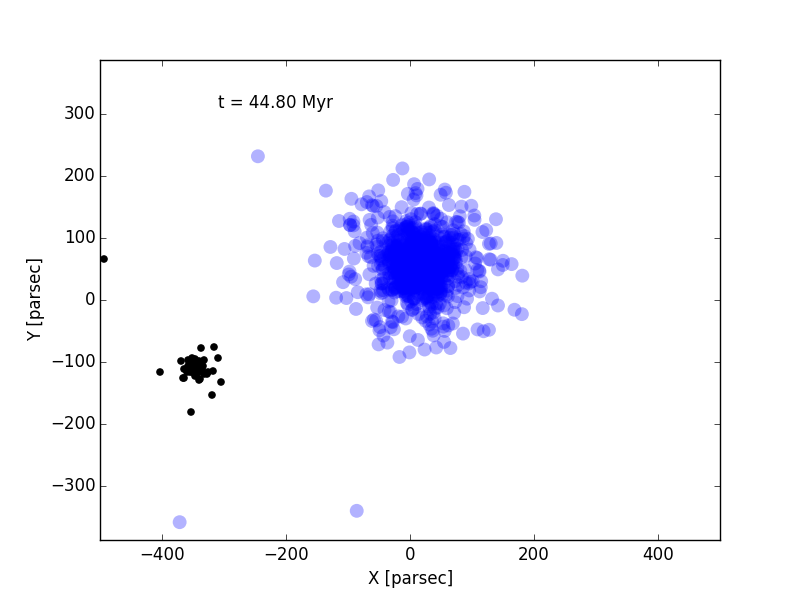
\includegraphics[width=\hsize]{img/test-44-8.png}
    \caption{Snapshot a stellar cluster (black) in orbit around a giant molecular cloud (blue, centered). The cloud is plotted transparent points because the dots indicate smoothed particle hydrodynamics particles representing regions of gas, not point masses.}\label{fig:GMC_with_cluster}
\end{figure}

The parameter space is varied as following. The values of $v_\infty$, in unit km/s, vary from 0.05 to 0.25 at intervals of 5, and from 0.25 to 3 with a step size of 0.25. For each $v_\infty$ value we simulate the impact parameter $d$, in unit parsec, from 5 to 15 incrementing with 5, and from 20 to 300 with 20 units between the data points. Within this range of $d$ and $v_\infty$ we obtain the interesting cases given in Table~\ref{tab:cases}, where the parameters can also be found and a reference to the end state of the simulation. Fig.~\ref{fig:v_25_d_280} to Fig.~\ref{fig:v_25_d5} show those end states. The previous paragraph also applies here.

%\textit{Vary the initial parameters of the simulation and produce an image of the following outcomes, if one is not possible, discuss why:}

\begin{table*}
    \caption{Interesting cases in the $d$,$v_\infty$-plane. Here $d$ is the impact parameter and $v_\infty$ is the initial cluster velocity placed at infinity. We have used AMUSE to simulate interactions of a stellar cluster using the BHTree algorithm with and a giant molecular cloud using the Fi smoothed particle hydrodynamics algorithm.}
    \label{tab:cases}
    \centering
    \begin{tabular}{l c c c}
        \hline\hline
        Case & $v_\infty$ & $d$ & Shown in \\
        \hline
        Both star cluster and GMC remain intact. & 0.25 & 280 & Fig.~\ref{fig:v_25_d_280} \\
        The star cluster is disrupted by the GMC. & 0.10 & 10 & Fig.~\ref{fig:v_10_d_10} \\
        The GMC is disrupted by the star cluster. & 0.15 & 20 & Fig.~\ref{fig:v_15_d_20} \\
        The star cluster takes some gas from the GMC. & 0.75 & 80 & Fig.~\ref{fig:v_75_d_80} \\
        The star cluster is captured and remains inside the GMC. & 0.25 & 5 & Fig.~\ref{fig:v_25_d_5} \\
        \hline
    \end{tabular}
\end{table*}

\begin{figure}[h!]
    \centering
    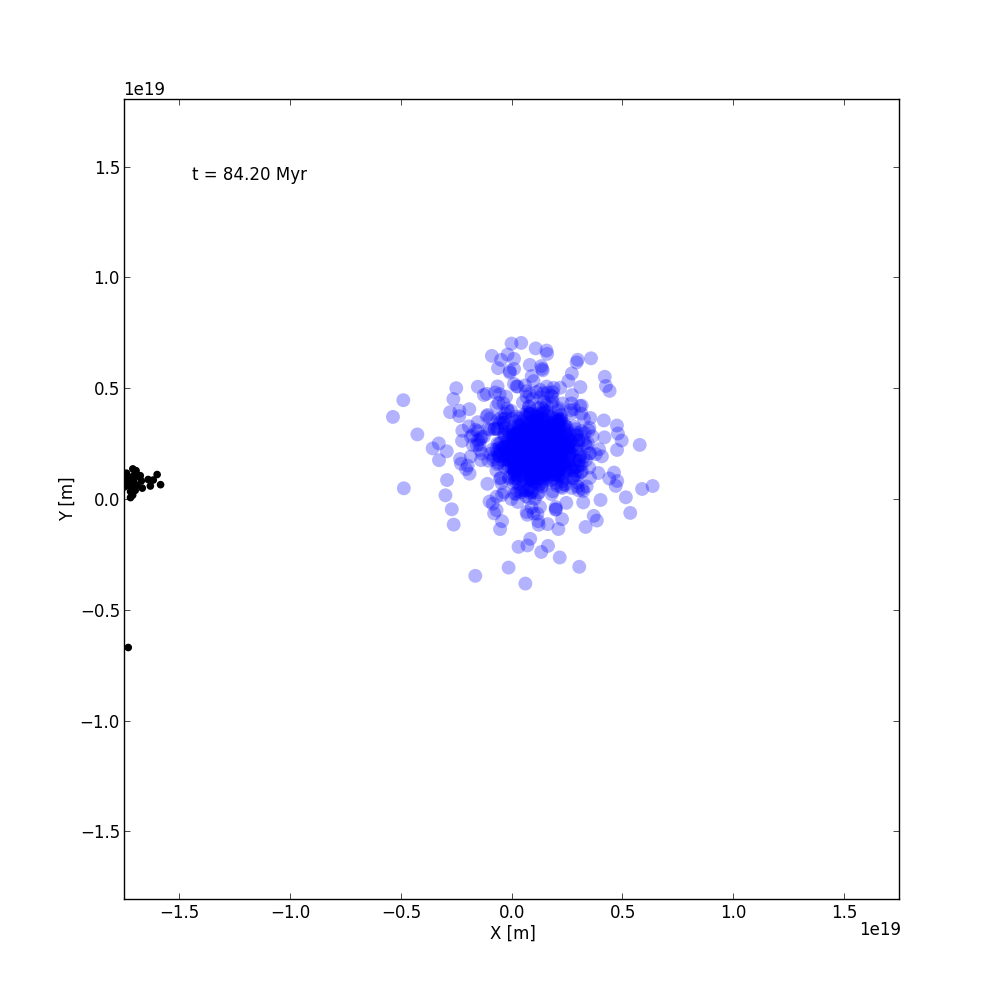
\includegraphics[width=\hsize]{img/v_25_d_280.png}
    \caption{Snapshot of a stellar cluster that has initial velocity at infinity $v_\infty = 0.25$ km/s and giant molecular cloud with impact parameter $d = 280$ parsec. From this image it can clearly be seen that both the cluster and the cloud remain intact. The end time of the simulation $t$ is indicated in the upper left corner.}\label{fig:v_25_d_280}.
\end{figure}
\begin{figure}[h!]
    \centering
    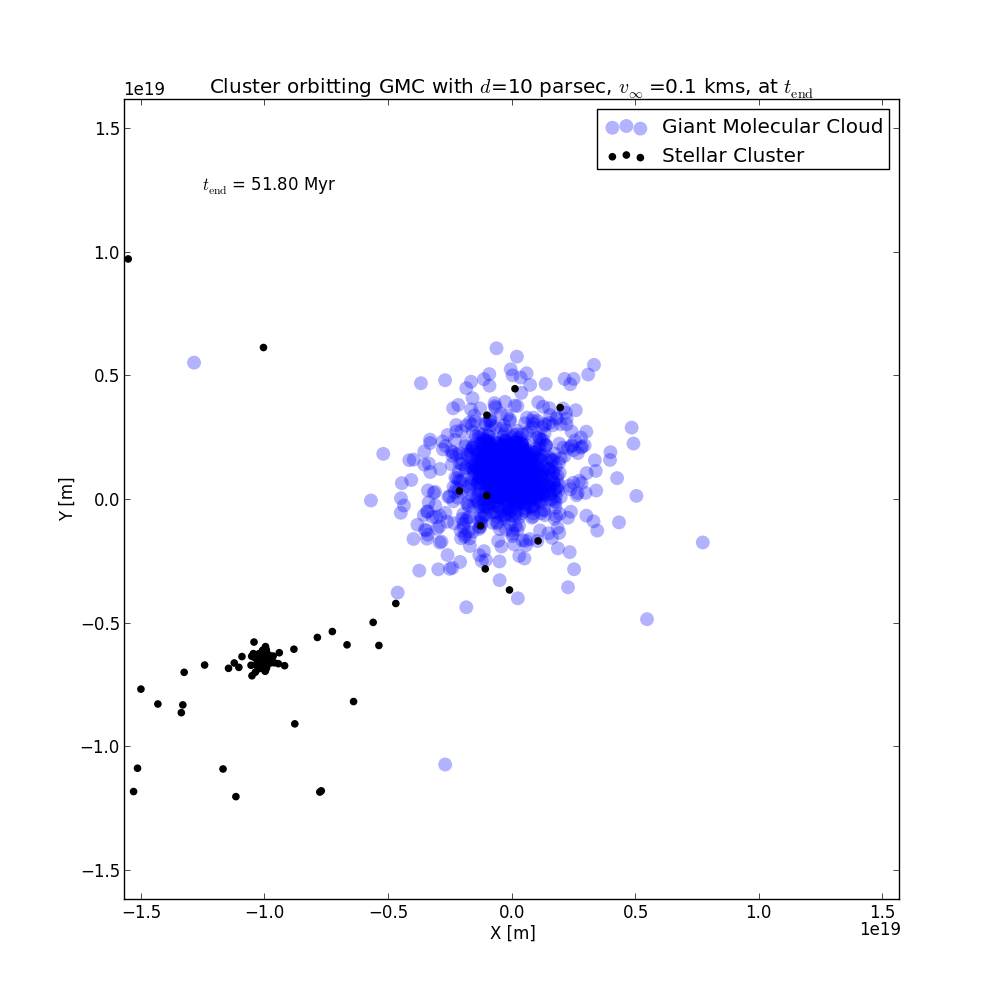
\includegraphics[width=\hsize]{img/v_10_d_10.png}
    \caption{Here $v_\infty = 0.10$ km/s and $d = 10$ parsec results in a disruption of the cluster by the cloud.}\label{fig:v_10_d_10}
\end{figure}
\begin{figure}[h!]
    \centering
    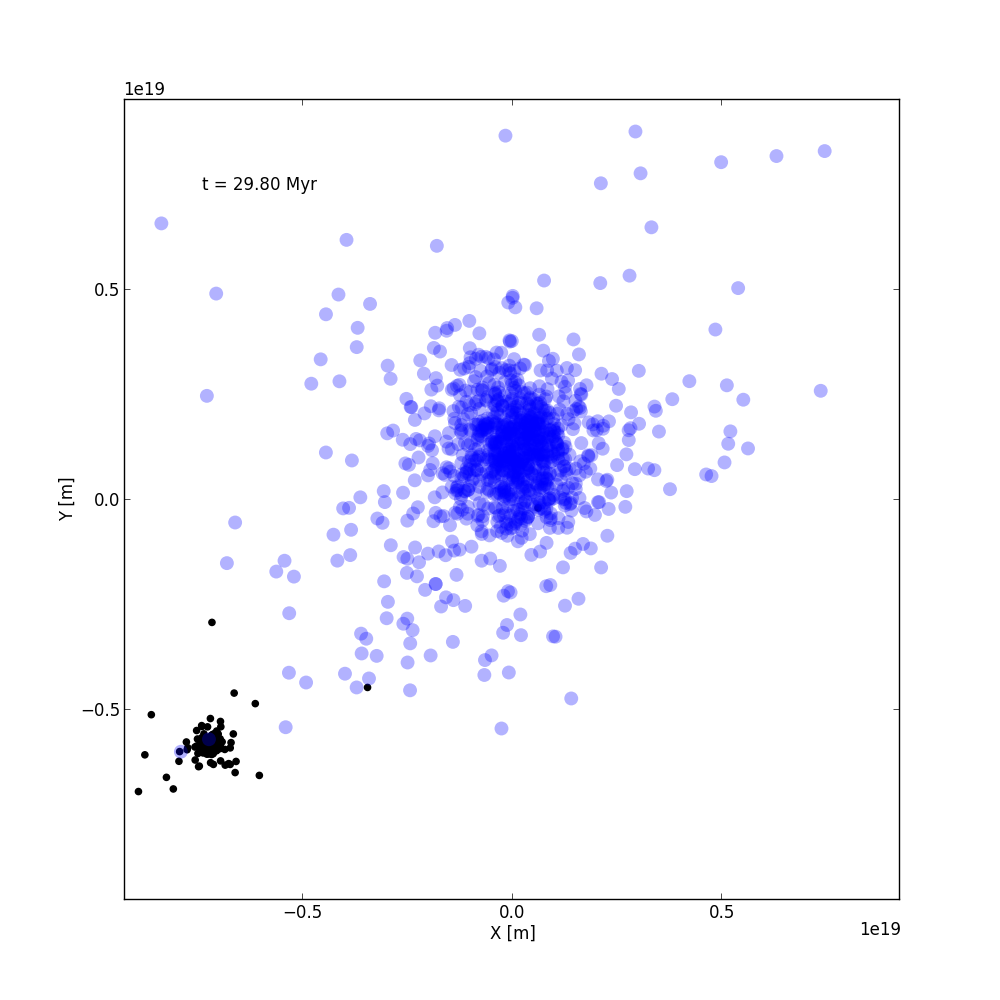
\includegraphics[width=\hsize]{img/v_15_d_20.png}
    \caption{With initial parameters $v_\infty = 0.15$ km/s and $d = 20$ parsec we observe that the cloud is disrupted by the cluster.}\label{fig:v_15_d_20}
\end{figure}
\begin{figure}[h!]
    \centering
    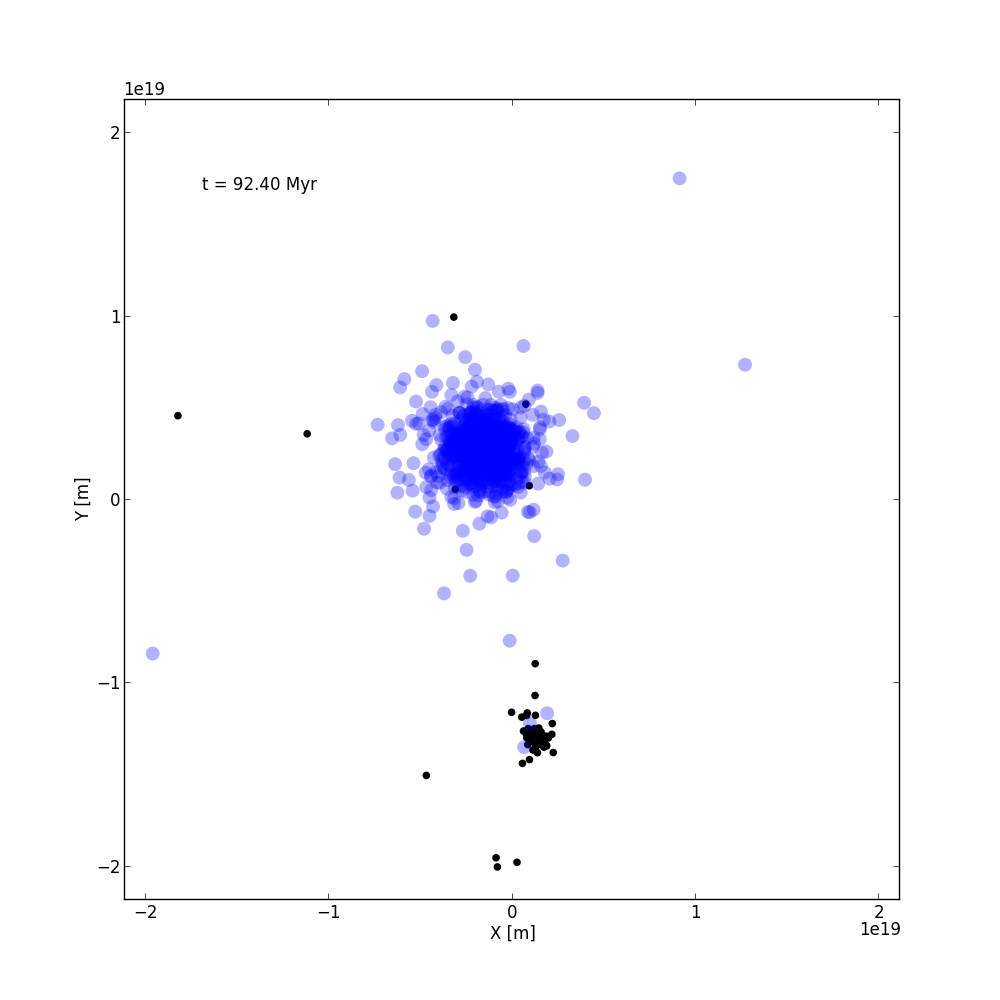
\includegraphics[width=\hsize]{img/v_75_d_80.png}
    \caption{Simulating with $v_\infty = 0.75$ km/s and $d = 80$ parsec it can be seen that some of the gas from the cloud is gravitationally bound by the cluster}\label{fig:v_75_d_80}
\end{figure}
\begin{figure}[h!]
    \centering
    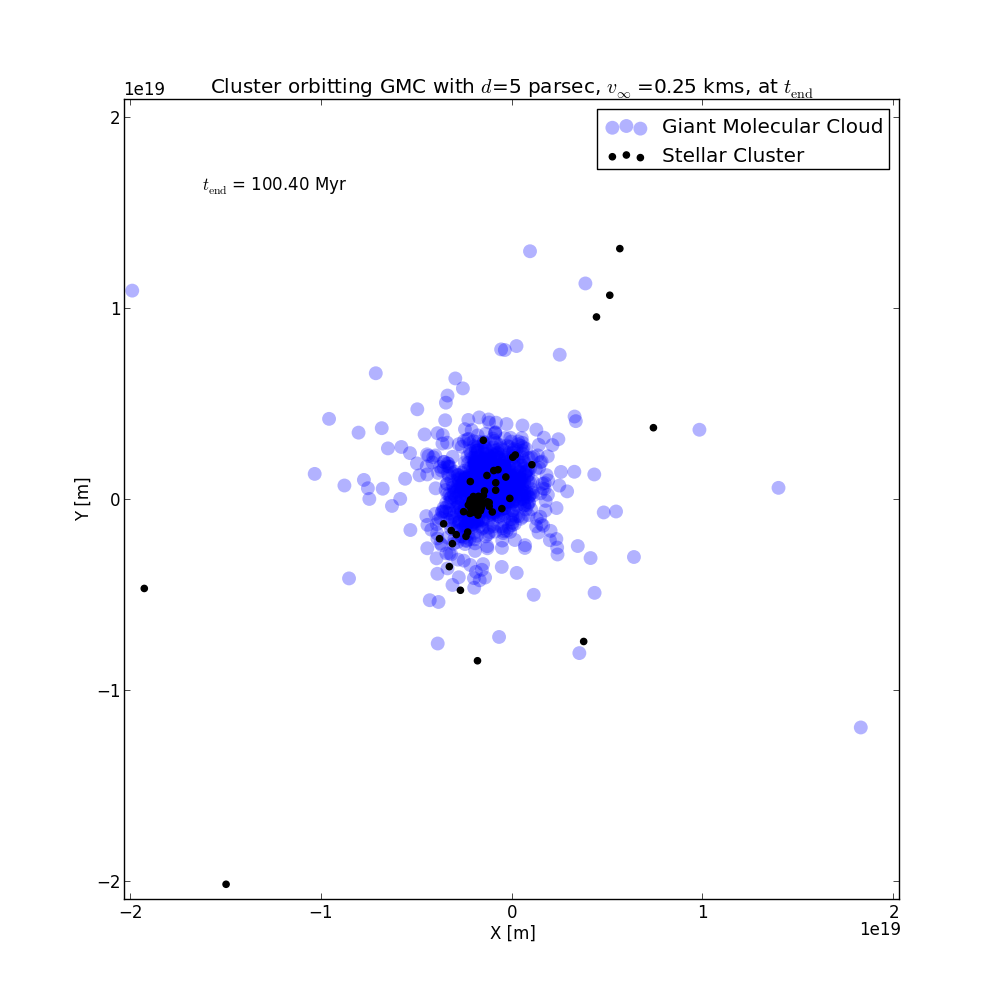
\includegraphics[width=\hsize]{img/v_25_d_5.png}
    \caption{Using $v_\infty = 0.25$ km/s and $d = 5$ parsec yields a partially captured cluster by the cloud. It is not clear from this image if the cluster is fully captures. This should be studied in greater detail prior to drawing conclusions.}\label{fig:v_25_d_5}
\end{figure}

The result in Fig.~\ref{fig:v_25_d_5} we find surprising. Our expectation is that the capture of the cluster by the GMC will not happen. Notice that this is merely a snapshot at one fixed point in time. The upper right stars seem to indicate that the cluster has been disrupted but it might not remain inside the GMC. This particular case requires a more elaborate analysis in order to conclude whether or not it stays inside the GMC. The reason for this expectation is REPLACE

\section{Multiple GMCs} \label{sec:multiplegmc}
Here we discuss the behaviour of the code when multiple molecular clouds are added to the system. This might be a more physically realistic setup. When a star cluster moves through its neighbourhood it may interact with not just one, but multiple gas clouds. To effectively simulate the cluster interacting with multiple distinct GMCs they need to be spaced far enough apart to not interact with each other. I.e. we do not want the GMCs to merge, otherwise the simulation is simulating a scenario where the cluster is still interacting with just one GMC, that just happens to be bigger. Ideally the cluster is really only interacting with one GMC in the simulation at a time. Adding the extra GMCs does add computational complexity. First of all the simulated time needs to be longer, because the time that the cluster is traveling in between the GMCs needs to be added; the simulation is not just simulating the time the cluster is actually interacting with a GMC anymore. This is dependent on the spacing in between GMCs, which is ideally large so that there is not too much interaction between GMCs. Making this distance too large however can blow up the simulation time.

% \textit{How does the computation time scale with the number of GMC's, assuming that each GMC has the same initial mass and number of particles.}
The second computational challenge is that even if the cluster is only interacting with one GMC at a time, adding the extra GMCs will have the hydrodynamics of the currently non-interacting GMCs be simulated as well during the entire simulation run. This adds overhead. Because adding extra GMCs to the simulation increases the number of years that need to be simulated, timing a full simulation run with different number of GMCs does not give full insight into this extra overhead. It may just be the extra simulation time added by the travel time between GMCs that is measured. Instead a fixed 4Myr simulation run is timed for simulations with one to ten GMCs. This is showcased in figure~\ref{fig:multi_GMCs_timings}, where it can be seen that the computation time for a set amount of simulated years increases linearly as more GMCs are added. This could be considered undesirable, because we're only interested in GMCs when they're interacting with the cluster. When they're not, their simulation could be wasted computational resources (given the important assumption that no significant change from the initial states of the GMCs occurs until they start interacting with the cluster).

Besides the computational challenges of having multiple GMCs in one simulation one also needs to set up the simulation in such a way that the cluster will in fact interact with the GMCs, rather than completely miss them. Ideally one would want to set up so that the impact parameter for each cluster-GMC encounter can be controlled. One approach could be to assume a hyperbolic orbit for the first GMC encounter. Based on that a escape path and escape velocity can be calculated. The escape velocity can be then be used as the $v_\infty$ for the next interaction and based on the calculated path the second GMC can be positioned. The same attributes can be calculated for the second encounter and be used to be place the third GMC, and so forth.

One huge issue with this approach is that the GMC-cluster encounters are not nice, clean gravitational encounters between point masses. In fact, that the entire motivation for running sophisticated simulations for these encounters. Thus the exact path and speed the cluster will take when exiting are hard to predict.  And each additional GMC encounter will compound to the error in the predicted path of the cluster. This is showcased in figure~\ref{fig:two_GMCs}. The second (left) GMC was put on the predicted path the star cluster would take after encountering the first (middle) GMC. In the end only two star took this predicted path.

One potential simplification that can be made is to place all GMCs beyond the first directly on the predicted exit path of the cluster based on the first GMC encounter. This would limit the error somewhat to the first predicted escape path. If this is somewhat accurate, it will end up interacting with the other GMCs. This is in fact how the simulation for figure~\ref{fig:two_GMCs} was set up. The big downside is that there is no control of the impact parameter of the encounters beyond the first one. And it is still not a guarantee for success, because the prediction based on the first interaction may still be wrong.

Instead we can go back to our assumption that nothing much interesting happens when a GMC is not interacting with the cluster and only simulate one interaction at a time, without the other GMCs being part of the simulation during said simulated encounters. After each encounter the end state of the cluster is taken and used as the start state of the cluster at the next encounter. This kills two birds with one stone: it lowers the computational overhead and it gives more direct control over setting up the parameters for the encounters.

\begin{figure}
    \centering
    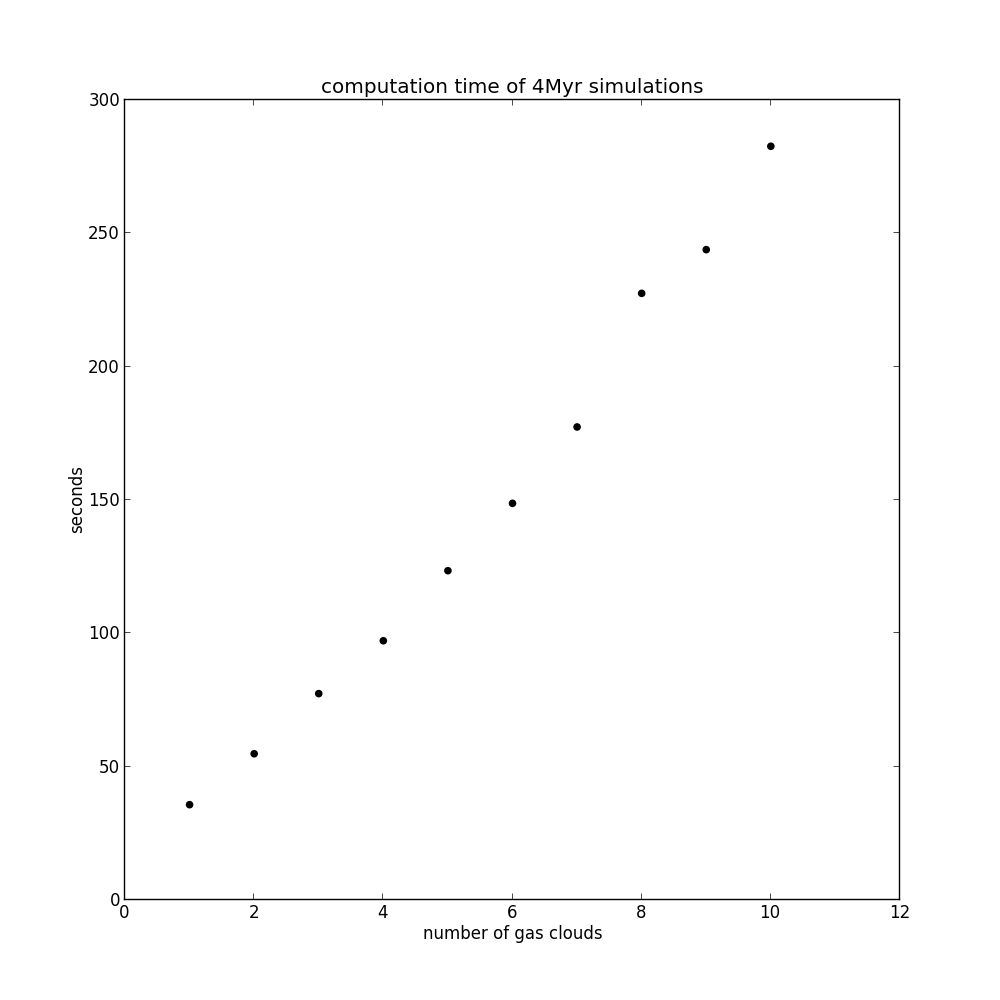
\includegraphics[width=\hsize]{img/multi_gmc_timings.png}
    \caption{Number of seconds that 4Myr simulation needs to run, showcasing a linear increase in the computation time as more GMCs are added to the simulation.}\label{fig:multi_GMCs_timings}
\end{figure}
\begin{figure}
    \centering
    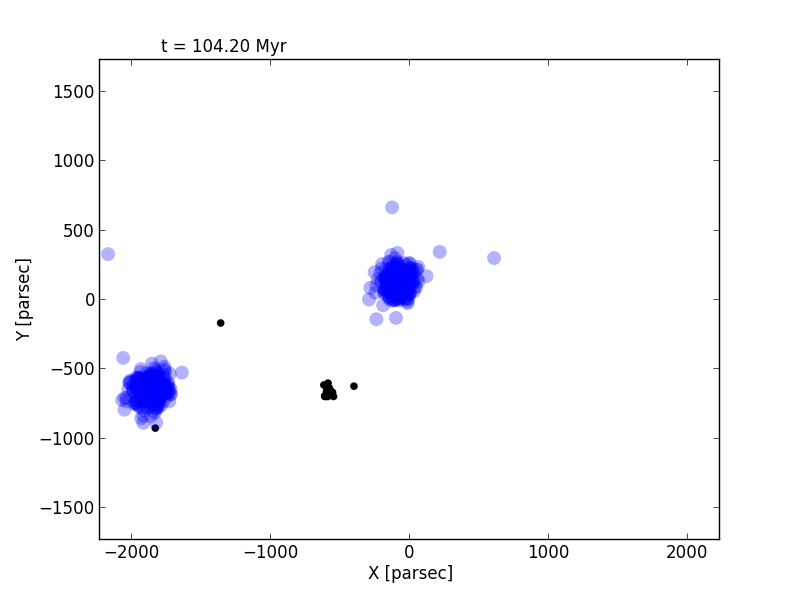
\includegraphics[width=\hsize]{img/two_gmcs_sim.png}
    \caption{Simulation of a cluster interacting with two GMCs}\label{fig:two_GMCs}
\end{figure}

\textit{The impact parameters ($d$ and $v_\infty$) between the star cluster and the first GMC are easy to choose. Discuss different methods to choose the impact parameters between the star cluster and the later clusters, what is the main challenge here?} REPLACE

\textit{Run simulations to find out when and how the second encounter is qualitatively different from a single encounter. Use the different scenarios from assignment 3C as a starting point.} REPLACE

\textit{Which changes in the star cluster's structural parameters can explain these differences.} REPLACE



\section{Discussion}\label{sec:discussion}

\section{Conclusions}\label{sec:conclusions}
\begin{enumerate}
    \item
    \item
    \item
    \item
\end{enumerate}


\begin{acknowledgements}
The authors are grateful for the help of their supervisors Edwin van der Helm, MSc and Prof. dr. S.F. Portegies Zwart. \\

This research has made use of NASA's Astrophysics Data System.
\end{acknowledgements}


%-------------------------------------------------------------------

\bibliographystyle{aa}
%\setlength{\bibsep}{0pt} % Remove whitespace in bibliography.
\bibliography{CA_Hydro_TLRH_s1603221_SS_s1617451_report_aa}
\end{document}
